% mnras_template.tex
%
% LaTeX template for creating an MNRAS paper
%
% v3.0 released 14 May 2015
% (version numbers match those of mnras.cls)
%
% Copyright (C) Royal Astronomical Society 2015
% Authors:
% Keith T. Smith (Royal Astronomical Society)

% Change log
%
% v3.0 May 2015
%    Renamed to match the new package name
%    Version number matches mnras.cls
%    A few minor tweaks to wording
% v1.0 September 2013
%    Beta testing only - never publicly released
%    First version: a simple (ish) template for creating an MNRAS paper

%%%%%%%%%%%%%%%%%%%%%%%%%%%%%%%%%%%%%%%%%%%%%%%%%%
% Basic setup. Most papers should leave these options alone.
\documentclass[a4paper,fleqn,usenatbib]{mnras}

% MNRAS is set in Times font. If you don't have this installed (most LaTeX
% installations will be fine) or prefer the old Computer Modern fonts, comment
% out the following line
\usepackage{newtxtext,newtxmath}
% Depending on your LaTeX fonts installation, you might get better results with one of these:
%\usepackage{mathptmx}
%\usepackage{txfonts}

% Use vector fonts, so it zooms properly in on-screen viewing software
% Don't change these lines unless you know what you are doing
\usepackage[T1]{fontenc}
\usepackage{ae,aecompl}

\usepackage{todonotes} %%% Remove afterwards


%%%%% AUTHORS - PLACE YOUR OWN PACKAGES HERE %%%%%

% Only include extra packages if you really need them. Common packages are:
\usepackage{graphicx}	% Including figure files
\usepackage{amsmath}	% Advanced maths commands
\usepackage{amssymb}	% Extra maths symbols

%%%%%%%%%%%%%%%%%%%%%%%%%%%%%%%%%%%%%%%%%%%%%%%%%%

%%%%% AUTHORS - PLACE YOUR OWN COMMANDS HERE %%%%%

% Please keep new commands to a minimum, and use \newcommand not \def to avoid
% overwriting existing commands. Example:
%\newcommand{\pcm}{\,cm$^{-2}$}	% per cm-squared

%%%%%%%%%%%%%%%%%%%%%%%%%%%%%%%%%%%%%%%%%%%%%%%%%%

%%%%%%%%%%%%%%%%%%% TITLE PAGE %%%%%%%%%%%%%%%%%%%

% Title of the paper, and the short title which is used in the headers.
% Keep the title short and informative.
\title[Power Spectrum Comparison...]{Power Spectrum Comparison... y ya veremos 
que mas!}

% The list of authors, and the short list which is used in the headers.
% If you need two or more lines of authors, add an extra line using \newauthor
\author[O. Nicol\'as Gomez-Giraldo, Juan C. Mu\~noz-Cuartas]{
O. Nicol\'as Gomez-Giraldo$^{1}$\thanks{E-mail: onicolas.gomez@udea.edu.co},
Juan C. Mu\~noz-Cuartas\thanks{E-mail: jcmunozc@udea.edu.co}
\\
% List of institutions
$^{1}$FACom - Instituto de F\'isica, FCEN, Universidad de Antioquia UdeA, Calle 
70 No. 52-21, Medell\'in, Colombia.\\}

% These dates will be filled out by the publisher
\date{Accepted XXX. Received YYY; in original form ZZZ}

% Enter the current year, for the copyright statements etc.
\pubyear{2015}

% Don't change these lines
\begin{document}
\label{firstpage}
\pagerange{\pageref{firstpage}--\pageref{lastpage}}
\maketitle

% Abstract of the paper
\begin{abstract}

Here we put the abstract

\end{abstract}

% Select between one and six entries from the list of approved keywords.
% Don't make up new ones.
\begin{keywords}
keyword1 -- keyword2 -- keyword3
\end{keywords}

\todo[inline,backgroundcolor=red!25]{\bf Objetivo del paper: Mostrar las 
bondades de la estimaci\'on del bispectrum usando Daubechies. En particular 
mostrando los efectos del aliasing en el bispectrum.}

%%%%%%%%%%%%%%%%%%%%%%%%%%%%%%%%%%%%%%%%%%%%%%%%%%%%%%%%%%%%%%%%%%%%%%
%% SECTION 1: Introduction
%%%%%%%%%%%%%%%%%%%%%%%%%%%%%%%%%%%%%%%%%%%%%%%%%%%%%%%%%%%%%%%%%%%%%%
\section{Introduction}
\todo[inline]{Presentaci\'on del problema. Resumen de la bibliograf\'ia. Qu\'e 
es lo que hacemos.  Por qu\'e es importante. Esquleto del paper}

Large Scale structure (LSS) of the Universe is thought to arise from the 
evolution of primordial fluctuations which are the result of gravitational 
instabilities at the early Universe (\textbf{cite}). In order to characterize 
quantitatively how is the clustering of these structures, different 
statistical methods are used to infer properties that can give constraints to 
cosmological models as well to cosmological parameters (\textbf{cite}). Because 
the statistical independence of the Fourier modes of a homogeneous random field, 
these statistics are expressed in Fourier space, which makes the study of such 
field easier \citep{Martinez2002}.

The matter power spectrum is one of the most common statistical measures of 
gravitational clustering. Its importance arises from the fact that, for a 
gaussian random field, the power spectrum describes completely its statistical 
properties (\textbf{cite}). However, a complete description for a non-gaussian 
distribution, which can be primordial or can emerge from non-linear processes, 
requires the use of higher order correlation functions \citep{Peebles1980}.

The bispectrum, had emerged as a standard probe of non-gaussianities in the LSS. 
The bispectrum is the lowest order indicator of non-Gaussinity in the primordial 
density field, which allows to constraint inflationary models and can give 
information about non-linear phenomena like structure formation and galaxy bias 
(\textbf{cite}). Despite its advantages, the estimation of the bispectrum is a 
task that is far from trivial. Due to its computational efficiency, it is common 
to use Fast Fourier Transforms in order to get different Fourier space 
statistics. Usually, computing power spectrum and bispectrum requires the 
interpolation of the density field in a cartesian grid. This  interpolation is 
done via a mass assignment scheme (MAS), which is a convolution of the density 
field with a window function. The finite sampling of the convolved density field 
introduces an additional effect known as ``aliasing'', which is significant near 
to the Nyquist wavevector and has to be corrected for a precise estimation 
\citep{HockneyEastwood1981,Jing2005,Jeong2010}.

%Qu\'e trabajos previos se han desarrollado al respecto?
\todo[inline,backgroundcolor=blue!25]{Power spectrum had been measured from 
most of the redshifts survey, although, in the bispectrum case had been 
estimated in a lower amount \textbf{(dar ejemplos de estimaciones en otros 
papers)}.}

%C\'ual es el problema con el MAS?
In addition, power spectrum and bispectrum are also extensively estimated from 
N-body simulations. For this case, because of the large amount of particles 
involved, it is necessary to use fast Fourier transform (FFT) algorithms. 
Consequently, it is necessary to sample the density field $\rho(\mathbf{x})$ on 
a regular grid. This sampling process is mathematically equivalent to doing a 
convolution $\rho(\mathbf{x}_p)=\left[\rho * W\right](\mathbf{x}_p)$, where the 
function $w(\mathbf{x})$ is known as window function and its functional form 
depends on the way (scheme) used to sample the discrete particle distribution 
to the regular grid points. Therefore, the value obtained with FFT is not equal 
to the result obtained with Fourier transform (FT), in order to get the proper 
values it is necessary to correct the effects involved by the sampling on the 
regular grid \citep{Jing2005,Cui2008}.

%Hablar del objetivo del art\'iculo.
In this work we are going to study the impact of the MAS in the estimation of 
the bispectrum, mainly taking in account the aliasing effect.
\todo[inline,backgroundcolor=blue!25]{poner estructura del articula}

Qu\'e es lo que se presenta nuevo en este trabajo? -> El impacto del MAS en 
$B(k_123)$.

%%%%%%%%%%%%%%%%%%%%%%%%%%%%%%%%%%%%%%%%%%%%%%%%%%%%%%%%%%%%%%%%%%%%%%
%% SECTION 2: OBSERVATIONAL DATA
%%%%%%%%%%%%%%%%%%%%%%%%%%%%%%%%%%%%%%%%%%%%%%%%%%%%%%%%%%%%%%%%%%%%%%
\section{Theory: Power spectrum, bispectrum and estimation} 
\todo[inline]{Teor\'ia b\'asica del $P(k)$ y $B(k1,k_2,k_3)$. Definiciones, 
estimadores (formalismo)} \label{sec:theory}

% Formally, the cosmic mass density field is described by the density function. 
% The knowledge of the value of the density field at every time during 
% Universe evolution and position would be the solution of the problem of 
% the evolution of structures at large scales \citep{Peacock1999}. However, 
% knowing such function would imply a full solution to the problem of structure 
% formation, which is impossible to solve analytically and hence, get the exact 
% function of the density field. It is possible to obtain approximate solutions 
% for idealized cases or for the linear growing regime 
% (\cite{Peebles1980,Bernardeau2002}), but the detailed solution of all the 
% process is obtained through numerical solutions.

In cosmology, matter distribution is described as a continuous function of 
space and time. To study the properties related with these fields, statistical 
tools are used, mainly because there is not direct observational access to the 
cosmological fluctuations, furthermore, the involved scale times are so big that 
there is not possible to track the temporal evolution of a single system 
\citep{Bernardeau2002,Martinez2002}.

Density fields had the properties of been statistically homogeneous and 
isotropic. 



%As a result of the recent galaxy surveys such as the Sloan Digital Sky Survey  
%(SDSS) \textbf{(citation Required)}, there has been possible to map the large 
%scale structure (LSS) of the Universe.

Knowledge of the distinct statistical properties at large scales can provide  
information about the nature of primordial overdensities, different possible 
inflationary scenarios, as well as give constrains on cosmological parameters 
and give information about different non linear phenomena such as gravity.


\subsection{Power spectrum}

The power spectrum $P(k)$ is the simplest Fourier statistic that allows to  
characterize the clustering pattern of the density field. It is the Fourier 
transform of the two point correlation function and can be defined from the 
density contrast in Fourier space $\delta(\mathbf{k}) = 
\int\exp(i\mathbf{k}\cdot\mathbf{r})\delta(\mathbf{r})\,\text{d}^3\mathbf{r}$ as
\begin{equation}
  \langle\delta(\mathbf{k}_1)\delta(\mathbf{k}_2)\rangle 
  = \left(2\pi\right)^3 P(k_1)\, \delta^D\left(\mathbf{k}_1+\mathbf{k}_2\right)
\end{equation}
where $\delta^D$ is the Dirac delta function and indicate the connected part 
between wavevectors $\mathbf{k}_1$ and $\mathbf{k}_2$, the symbol 
$\langle\cdots\rangle$
denotes the ensemble average over independent realizations of the Universe. 
Under the ergodicity hypothesis the average over different directions of the 
$\mathbf{k}$ will give the same result as the ensemble average 
\citep{GilMarin2012}.

For the density contrast field $\delta$, the total variance can be written as
\begin{equation}
  \sigma^2 = 4\pi \int_0^\infty P(k) \frac{k^2}{(2\pi)^3}\text{d}k,
\end{equation}
letting us to show an alternative form of the power spectrum also popular in 
cosmology
\begin{equation}
  \Delta^2(k) = \frac{1}{2\pi} P(k) k^3,
\end{equation}
accordingly, we can write the variance of the field as
\begin{equation}
  \sigma^2 = \int_0^\infty \Delta^2(k) \text{d}\left(\ln k\right).
\end{equation}

The power spectrum describes the second moment of a random field $\delta$ and 
represents an initial tool to characterize the clustering at large scales. For 
a Gaussian random field, the power spectrum describes completely its 
statistical features. The galaxy power spectrum had been extensively used in 
the literature to constraint structure formation, cosmological parameters as 
well as galaxy bias models, giving valuable information that helped to 
establish the $\Lambda$CDM as the standard cosmological model 
\citep{GilMarin2012} \textbf{(Poner otras citas ac\'a)}.

\subsection{Bispectrum}

When a random field is not Gaussian, is necessary to use higher order 
correlation functions in order the characterize the statistical properties 
of this field. The next statistic of interest is the bispectrum or the three 
point correlation function in Fourier space, which can be written as
\begin{equation}
  \left\langle \delta(\mathbf{k}_1) \delta(\mathbf{k}_2) \delta(\mathbf{k}_3) 
  \right\rangle = \left(2\pi\right)^3 
  \delta^D\left(\mathbf{k}_1+\mathbf{k}_2+\mathbf{k}_3\right) B(k_1,k_2,k_3).
\end{equation}
In this case, the Dirac delta function demands that the bispectrum is non-zero 
only for wavevector configurations that make closed triangles, i.e.,
$\mathbf{k}_1+\mathbf{k}_2+\mathbf{k}_3=0$. 
It is important to note that the product 
$\delta(\mathbf{k}_1)\delta(\mathbf{k}_2)\delta(\mathbf{k}_3)$ is in general
a complex number, but once the mean is taken, the imaginary part goes to zero 
\citep{GilMarin2012}. 

It is usual to define the reduced bispectrum $Q$ by
\begin{equation}
  Q(k_1,\, k_2,\, k_3)
  =\frac{B(k_1,\, k_2,\, k_3)}{P(k_1)P(k_2)+P(k_2)P(k_3)+P(k_3)P(k_1)},
\end{equation}
even this quantity does not give any additional information to the power 
spectrum and bispectrum it had been of historical used in cosmology because is 
the associated hierarchical amplitude for the bispectrum and is weakly 
dependent on cosmology and scale.

For a Gaussian random field bispectrum is null, therefore, it can be used as an 
initial tool to observe non-primordial Gaussinity. In addition, whether or 
not the random field is initially Gaussian or not, when non-linear processes 
(such as gravitational collapse) are present, they introduce non-gaussianities, 
allowing bispectrum to be used to extract information about non-linearities 
in the galaxy clustering. Besides, galaxy biasing also introduce non-linear 
effects in the density field, letting us to use bispectrum as an important tool 
to study galaxy bias at large scales \citep{Matarrese1997,GilMarin2015}.


\subsection{Basic estimators}

For the power spectrum the basic estimator is built by using direct sampling. 
This consists on taking the average of the complex magnitude of the density
contrast in Fourier space in all the Fourier modes inside of a spherical shell 
of radius $k$ and width $\Delta k= s\,k_F$, were $k_F=2\pi/L$ is known as the 
fundamental frequency (for a comprehensive review of power spectrum and 
bispectrum estimation see \cite{Jeong2010}). With this, the estimator is given
by
\begin{equation}
  P^d(k) = \frac{V_F}{(2\pi)^3} \left( \frac{1}{N_{q}}
  \sum_{k-\frac{\Delta k}{2} < |\mathbf{q}| < k + \frac{\Delta k}{2}}
  |\delta(\mathbf{q})|^2 \right) \label{eq:PkEstimator}
\end{equation}
where $N_k$ is the number of elements inside the selected shell and $V_F=k_F^3$.

The bispectrum estimator is given as the ensemble average of all the possible  
triangles with sides $k_1,\,k_2,\,k_3$. Therefore, the estimator is given as
\begin{equation}
  B^d(k_1,k_2,k_3) = \frac{V_F}{(2\pi)^3}
  \left( 
  \frac{1}{N_\text{Tri}} 
  \sum_{q \in \text{Tri}_{123}} 
  \delta(\mathbf{q}_1) \delta(\mathbf{q}_2) \delta(\mathbf{q}_3) 
  \right) \label{eq:BkEstimator}
\end{equation}
where $\text{Tri}_{123}$ is the set of points $\{\mathbf{q}_1, \mathbf{q}_2, 
\mathbf{q}_3\}$ satisfying simultaneously that its magnitude is $k_i-{\Delta 
k}/{2} < |\mathbf{q}_i| < k_i+{\Delta k}/{2}$ and form a triangle, i.e.,
$\mathbf{q}_1 + \mathbf{q}_2 + \mathbf{q}_3 = \mathbf{0}$, $N_\text{Tri}$ is 
the number of elements of $\text{Tri}_{123}$.


\subsection{Shot noise}

The shot noise is an additional term introduced as a consequence of the 
discrete sampling of the density field. Therefore, because of the discrete 
nature of the particle distribution in N-body simulations, it is necessary to 
correct the shot noise effect by substracting it from the power spectrum and 
bispectrum. The shot noise for the power spectrum and bispectrum is respectively
\begin{equation}
  P_{SN}(k) = \frac{1}{\bar{n}} \label{eq:PSN},
\end{equation}
\begin{equation}
  B_{SN}(k_1,k_2,k_3) = \frac{1}{\bar{n}} 
  \left[ P(k_1) + P(k_2) + P(k_3) \right] + \frac{1}{\bar{n}^2} \label{eq:BSN},
\end{equation}
where $\bar{n}$ is the number density of particles. Hence, the basic shot noise 
corrected estimators are given as
\begin{equation}
  P(k)=P^d(k) - P_{SN}(k)
\end{equation}
\begin{equation}
  B(k_1,k_2,k_3)=B^d(k_1,k_2,k_3)-B_{SN}(k_1,k_2,k_3).
\end{equation}

%%%%%%%%%%%%%%%%%%%%%%%%%%%%%%%%%%%%%%%%%%%%%%%%%%%%%%%%%%%%%%%%%%%
%Teoria basica del Pk y Bk. Definiciones, estimadores (formalismo)%
%%%%%%%%%%%%%%%%%%%%%%%%%%%%%%%%%%%%%%%%%%%%%%%%%%%%%%%%%%%%%%%%%%%


\subsection{Mass assignment scheme: NGP, CIC, TGP, Deaubichis}
\label{sec:theory:MAS}

\todo[inline]{Teor\'ia b\'asica del MAS. Definiciones, estimadores (formalismo). 
Implicaciones ventajas y desventajas de cada m\'etodo.}

For computational efficiency, statistics in Fourier space are usually calculated 
by making use of fast Fourier transform (FFT), in which is required a 
``sampling'' on a regular grid of the overdensities values. From a practical 
standpoint this is equivalent to the convolution of the density contrast with a 
window function $W(\mathbf{k})$, defined by an assignation scheme [MAS; 
\cite{HockneyEastwood1981}]. Once the overdensities in Fourier space are  
calculated power spectrum and bispectrum can measured through different 
estimators [\textit{e.g.} \citet{Jeong2010,Scoccimarro1998}].

The most common mass assignment schemes used are the Nearest Grid Point (NGP),
Cloud In Cell (CIC) and Triangular Shaped Cloud (TSC), whith the window function 
given as $W(\mathbf{r})=\prod_{i=1}^3 W(x_i)$, where
\citep{HockneyEastwood1981}
\begin{equation}
  W_{NGP}(x) =\frac{1}{H}
  \begin{cases}
    1   & \quad \text{if } |x| < H/2\\
    1/2 & \quad \text{if } |x| = H/2\\
    0   & \quad \text{otherwise}
  \end{cases}
\end{equation}
\begin{equation}
  W_{CIC}(x) = \frac{1}{H}
  \begin{cases}
    1 - |x|/H & \quad \text{if } |x| < H\\
    0         & \quad \text{otherwise}
  \end{cases}
\end{equation}
\begin{equation}
  W_{TSC}(x)=\frac{1}{H}
  \begin{cases}
    \frac{3}{4} - \left(\frac{x}{H}\right)^2          & \quad \text{if } 
    |x| \leq \frac{H}{2}\\
    \frac{1}{2}\left(\frac{3}{2}-\frac{|x|}{H}\right) & \quad \text{if } 
    \frac{H}{2} \leq |x| \leq \frac{3H}{2}\\
    0                                                 & \quad \text{otherwise},
  \end{cases}
\end{equation}
where $H$ is the grid spacing. In addition, 
In the Figure \ref{fig:MASplot} we plot the different forms of these 
window functions.

\begin{figure}
  \centering
  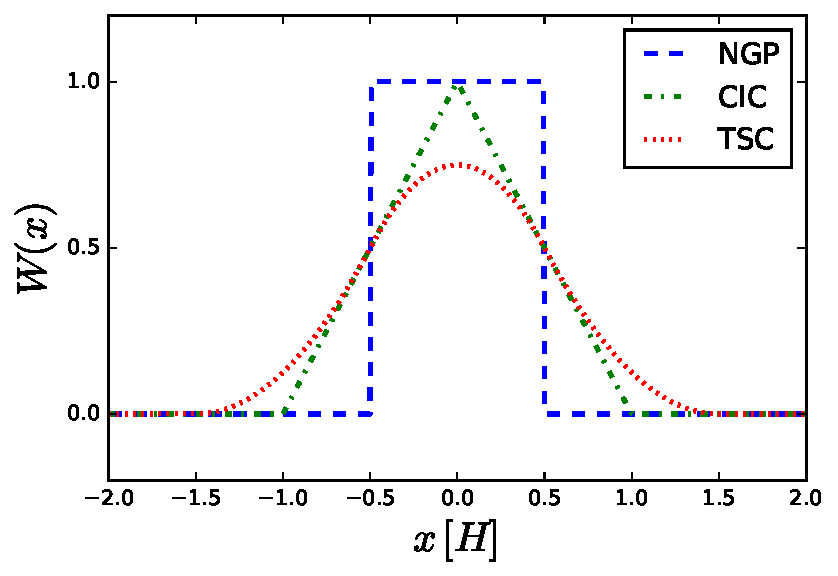
\includegraphics[width=0.9\columnwidth]{images/MAS_plots.pdf}
  \caption{Graphic of the most common mass assignment schemes.}\label{fig:MASplot}
\end{figure}

Given a wavevectors $\mathbf{k}=(k_1,\,k_2,\,k_3)$, the Fourier transform of 
the window functions for 
the different mass assignment schemes are given as a product of the Fourier transform for each
component
\begin{eqnarray}
  W(\mathbf{k}) &=& \prod_{i=1}^3 W(k_i) \nonumber\\
  &=& \left[ \prod_{i=1}^3 \frac{\sin\left(\pi k_i/ 2 k_N \right)}{\pi k_i / 2 k_N} \right]^p
\end{eqnarray}
where $p=1$ for NGP, $p=2$ for CIC and $p=3$ for TSC. In the Figure 
\ref{fig:MAS_FT} we show the Fourier transform of the window functions in terms
of $k_N$, we can see how for the NGP scheme it has appreciable values for 
values even bigger than $5 k_N$ while in the CIC scheme for values $k\gtrsim 
3 k_N$ it drops and for the TSC when $k\gtrsim 
2 k_N$ it goes to zero.

\begin{figure}
  \centering
  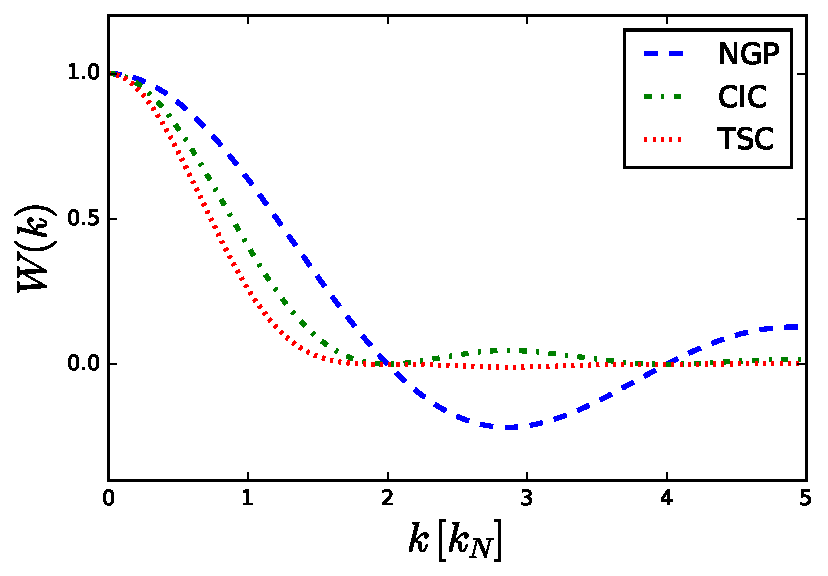
\includegraphics[width=0.9\columnwidth]{images/MAS_FT.pdf}
  \caption{Graphic of the Fourier transform for the most common mass assignment schemes.}
  \label{fig:MAS_FT}
\end{figure}

% \begin{figure}
%   \centering
%   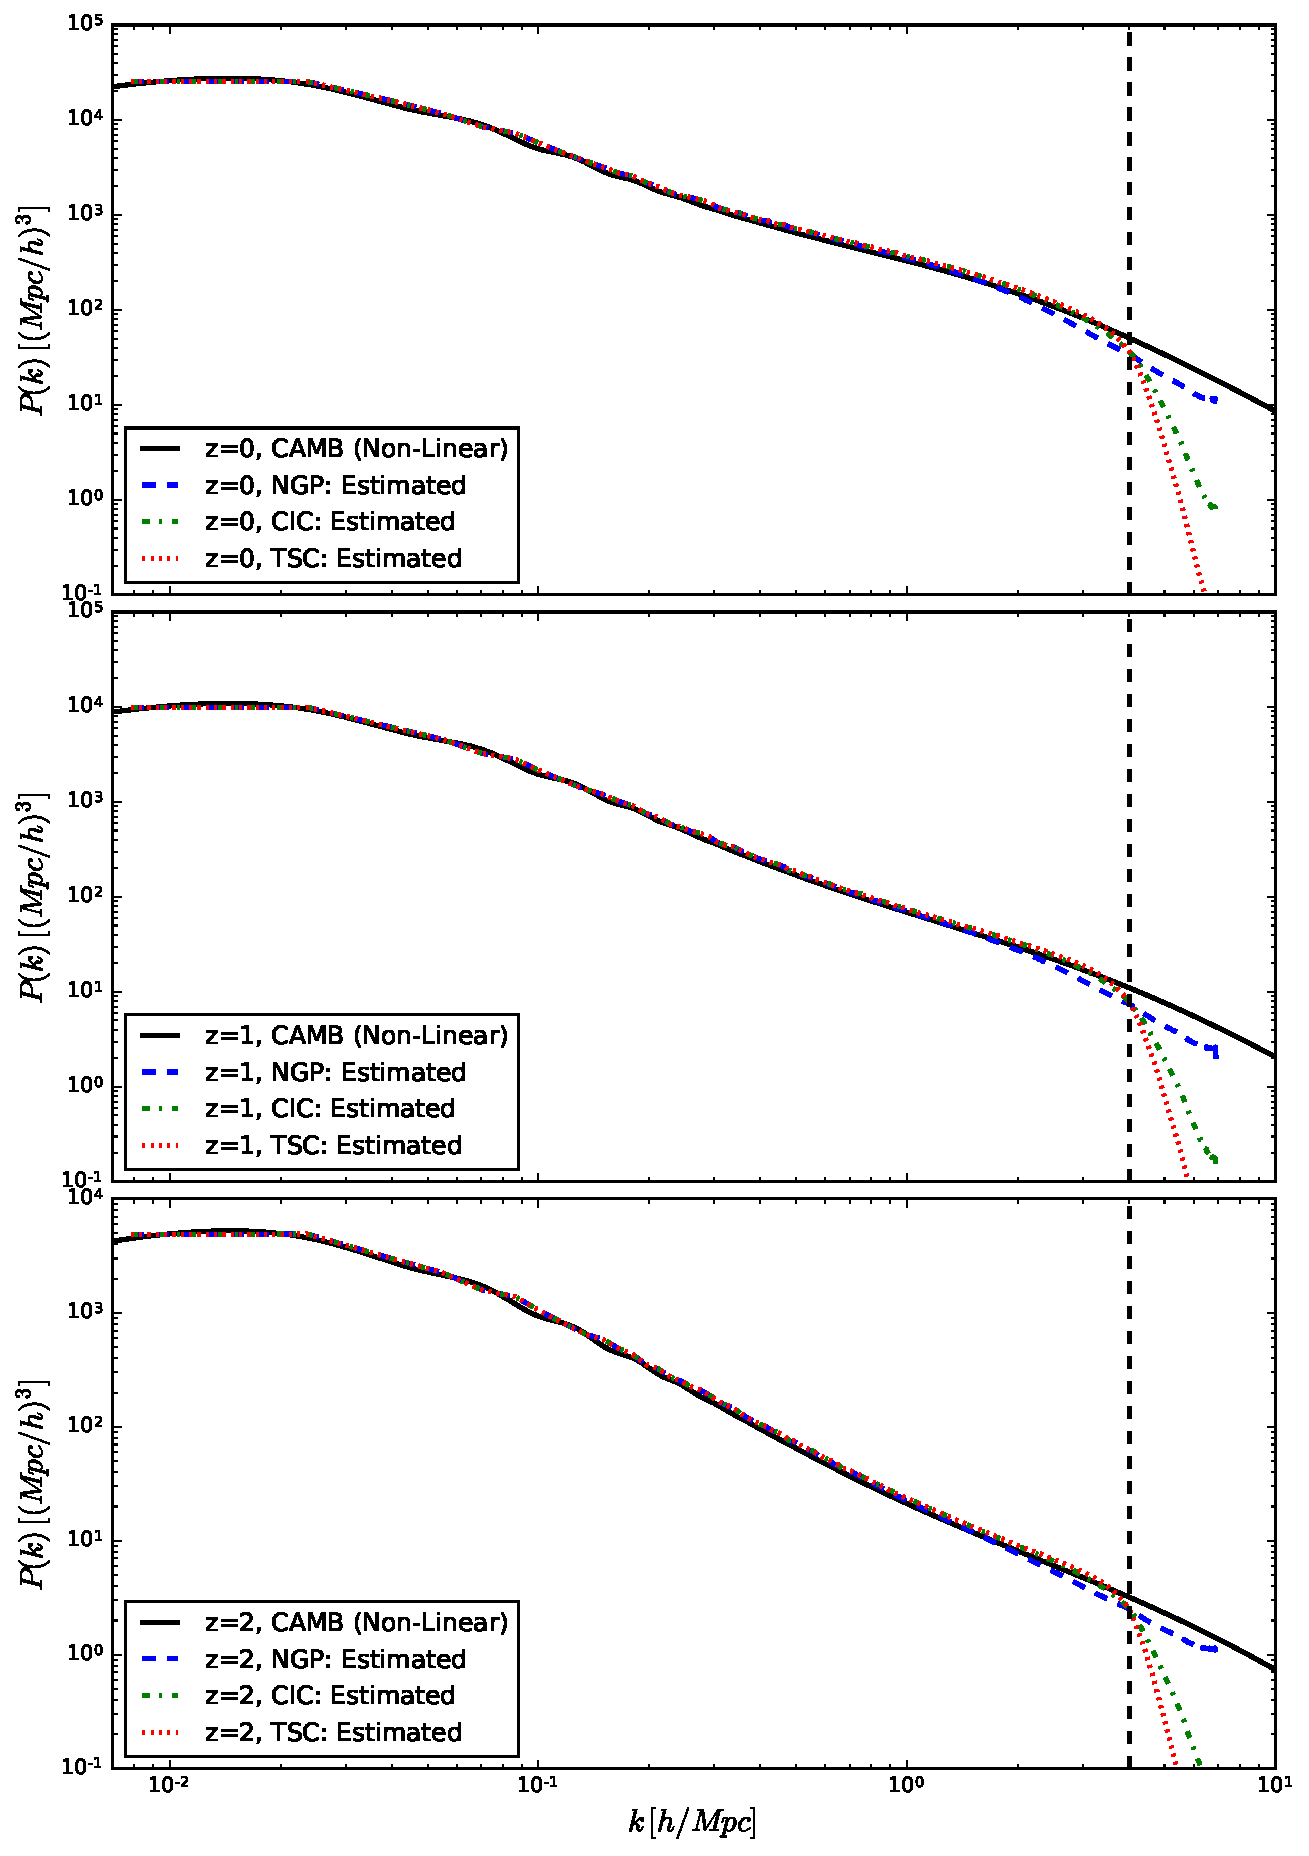
\includegraphics[width=1\columnwidth]{images/NGP_CIC_TSC_VS_CAMB_ONECOLUMN.pdf}
%   \caption{The aliasing effect in the power spectrum estimation for the most
%   common schemes.}\label{fig:MASeffects}
% \end{figure}

\todo[inline]{(Figura: figurita con las formas!)}


\subsection{Aliasing for the power spectrum and bispectrum}
\label{sec:theory:aliasing}

In a practical sense, a mass assignment scheme is equivalent to a convolution of 
the density contrast with a window function (in which the particular form is 
defined by the scheme used). There is an effect introduced in the estimations 
of the power spectrum, bispectrum and their respective shot noise terms known 
as aliasing, which makes that the different modes in Fourier space lost its
independence \citep{HockneyEastwood1981,Jing2005}.

\cite{Jing2005} derived the power spectrum estimator when using FFT to get the 
desity constrast in Fourier space $\delta^f(\mathbf{k})$ as
\begin{eqnarray}
  \left\langle\left|\delta^f(\mathbf{k})\right|^2\right\rangle 
  &=& \sum_\mathbf{n} 
  \left|W(\mathbf{k}+2k_N\mathbf{n})\right|^2\,P(\mathbf{k}+2k_N\mathbf{n}) \nonumber \\
  & & +\frac{1}{\bar{n}} \sum_\mathbf{n} \left|W(\mathbf{k}+2k_N\mathbf{n})\right|^2, \label{eq:JingAliasing}
\end{eqnarray}
where $W(\mathbf{k})$ is the FT of the window function $W(\mathbf{r})$, $k_N=\pi/H$ is the Nyquist 
wavevectors and the summation is over the three dimensional integer vectors 
$\mathbf{n}$. Here we are 
going to deduce the alias effect but for the bispectrum.

By using FFT, the density contrast in Fourier space is given as \citep{Jing2005}
\begin{equation}
  \delta^f(\mathbf{k}) = \frac{1}{\bar{n}}\sum_\mathbf{g} n^f(\mathbf{r}_g)\exp(i\mathbf{r}_g\cdot\mathbf{k})
  -\delta^\text{K}_{\mathbf{k},\mathbf{0}} \label{eq:deltaf},
\end{equation}
where the superscript $f$ means that the quantity was fast Fourier transformed, $n^f(\mathbf{r}_g)$
is the density convolved by the window function at the $\mathbf{g}$th grid point 
$\mathbf{r}_g=\mathbf{g}H$, here $\mathbf{g}$ is an integer vector,
\begin{equation}
  n^f(\mathbf{r}_g) = \int n(\mathbf{r}) 
  W(\mathbf{r}-\mathbf{r}_g)\,\text{d}^3\mathbf{r}, \label{eq:nf}
\end{equation}
where $\delta^\text{K}$ is the Kronecker delta.

Equation (\ref{eq:nf}) can be expressed in a different way by using the sampling 
function
$\Pi(\mathbf{r})$ which is defined as
\begin{equation}	
  \Pi(\mathbf{r}) = \sum_\mathbf{n} \delta^D(\mathbf{r}-\mathbf{n}).
\end{equation}
Defining a new convolved particle density
\begin{equation}
  n'^f(\mathbf{r}) = \Pi\left(\frac{\mathbf{r}}{H}\right) \int n(\mathbf{r}_1) 
  W(\mathbf{r}_1-\mathbf{r})\,\text{d}^3\mathbf{r}_1,
\end{equation}
is possible to construct
\begin{equation}
  \delta'^f(\mathbf{k}) = \frac{1}{\bar{n}}
  \int n'^f(\mathbf{r})\exp(i\mathbf{r}\cdot\mathbf{k})\,\text{d}^3\mathbf{r}
  -\delta^\text{K}_{\mathbf{k},\mathbf{0}} \label{eq:deltaf},
\end{equation}
we have that \citep{Jing2005}
\begin{equation}
 \delta'^f(\mathbf{k})=\delta^f(\mathbf{k}),
\end{equation}
therefore, the alternative form of equation (\ref{eq:deltaf}) is
\begin{equation}
  \delta^f(\mathbf{k}) = \frac{1}{\bar{n}}
  \int \Pi\left(\frac{\mathbf{r}}{H}\right) \sum_i n_i W(\mathbf{r}_i-\mathbf{r})\exp(i\mathbf{r}\cdot\mathbf{k})\,\text{d}^3\mathbf{r}
  -\delta^\text{K}_{\mathbf{k},\mathbf{0}}.
\end{equation}
The three point ensemble average is given as

\begin{minipage}{1\columnwidth}
\onecolumn
% \begin{eqnarray}
%   \langle \delta^f(\mathbf{k}_1) \delta^f(\mathbf{k}_2) \delta^f(\mathbf{k}_3) \rangle &=&
%   \frac{1}{\bar{n}^3}\int \Pi\left(\frac{\mathbf{r}_1}{H}\right) 
%   \Pi\left(\frac{\mathbf{r}_2}{H}\right) \Pi\left(\frac{\mathbf{r}_3}{H}\right) \nonumber\\
%   && \times [ \sum_{i,j,k} \langle n_i n_j n_k \rangle W(\mathbf{r}_{i1}) W(\mathbf{r}_{j2}) W(\mathbf{r}_{k3}) \nonumber\\
%   && e^{i \mathbf{r}_1\cdot\mathbf{k}_1 + i \mathbf{r}_2\cdot\mathbf{k}_2 + i \mathbf{r}_3\cdot\mathbf{k}_3}
%   \text{d}^3\mathbf{r}_1 \text{d}^3\mathbf{r}_2 \text{d}^3\mathbf{r}_3 \nonumber\\
%   &+& \frac{1}{\bar{n}^2}\int 
%   \Pi\left(\frac{\mathbf{r}_1}{H}\right) \Pi\left(\frac{\mathbf{r}_2}{H}\right) \Pi\left(\frac{\mathbf{r}_3}{H}\right)
%   \langle n_i n_j n_k \rangle \nonumber\\
%   && W(\mathbf{r}_{i1}) W(\mathbf{r}_{j2}) W(\mathbf{r}_{k3}) \nonumber\\
%   && e^{i \mathbf{r}_1\cdot\mathbf{k}_1 + i \mathbf{r}_2\cdot\mathbf{k}_2 + i \mathbf{r}_3\cdot\mathbf{k}_3}
%   \text{d}^3\mathbf{r}_1 \text{d}^3\mathbf{r}_2 \text{d}^3\mathbf{r}_3   
% \end{eqnarray}
%\begin{onecolumn}
\begin{align}
  \langle \delta^f(\mathbf{k}_1) \delta^f(\mathbf{k}_2) \delta^f(\mathbf{k}_3) \rangle =&
  \frac{1}{\bar{n}^3}\int \Pi\left(\frac{\mathbf{r}_1}{H}\right) 
  \Pi\left(\frac{\mathbf{r}_2}{H}\right) \Pi\left(\frac{\mathbf{r}_3}{H}\right) \nonumber\\
  &\times \left[ \sum_{i\neq j\neq k} \langle n_i n_j n_k \rangle 
  W(\mathbf{r}_{i1}) W(\mathbf{r}_{j2}) W(\mathbf{r}_{k3}) \right.\nonumber \\
  &+\sum_{i=j,i\neq k} \langle n_i^2 n_k \rangle W(\mathbf{r}_{i1}) W(\mathbf{r}_{i2}) W(\mathbf{r}_{k3})
  +\sum_{i=k,i\neq j} \langle n_i^2 n_j \rangle W(\mathbf{r}_{i1}) W(\mathbf{r}_{j2}) W(\mathbf{r}_{i3})
  \left. +\sum_{j=k,i\neq j} \langle n_i n_j^2 \rangle W(\mathbf{r}_{i1}) W(\mathbf{r}_{j2}) W(\mathbf{r}_{j3})\right] \nonumber\\
  & \times e^{i \mathbf{r}_1\cdot\mathbf{k}_1 + i \mathbf{r}_2\cdot\mathbf{k}_2 + i \mathbf{r}_3\cdot\mathbf{k}_3}
  \text{d}^3\mathbf{r}_1 \text{d}^3\mathbf{r}_2 \text{d}^3\mathbf{r}_3 \nonumber\\
  &- \frac{1}{\bar{n}^2}\int \Pi\left(\frac{\mathbf{r}_1}{H}\right) \Pi\left(\frac{\mathbf{r}_2}{H}\right)
  \left[\sum_{i\neq j} \langle n_i n_j \rangle W(\mathbf{r}_{i1}) W(\mathbf{r}_{j2})
  +\sum_{i} \langle n_i^2 \rangle W(\mathbf{r}_{i1}) W(\mathbf{r}_{i2}) \right] e^{i \mathbf{r}_1\cdot\mathbf{k}_1 + i \mathbf{r}_2\cdot\mathbf{k}_2} \,
  \delta^K_{\mathbf{k}_3,\mathbf{0}}\,\text{d}^3\mathbf{r}_1 \text{d}^3\mathbf{r}_2 \nonumber\\
  &- \frac{1}{\bar{n}^2}\int \Pi\left(\frac{\mathbf{r}_1}{H}\right) \Pi\left(\frac{\mathbf{r}_3}{H}\right)
  \left[\sum_{i\neq k} \langle n_i n_k \rangle W(\mathbf{r}_{i1}) W(\mathbf{r}_{k3})
  +\sum_{i} \langle n_i^2 \rangle W(\mathbf{r}_{i1}) W(\mathbf{r}_{i3}) \right] e^{i \mathbf{r}_1\cdot\mathbf{k}_1 + i \mathbf{r}_3\cdot\mathbf{k}_3} \,
  \delta^K_{\mathbf{k}_2,\mathbf{0}}\,\text{d}^3\mathbf{r}_1 \text{d}^3\mathbf{r}_3 \nonumber\\
  &- \frac{1}{\bar{n}^2}\int \Pi\left(\frac{\mathbf{r}_2}{H}\right) \Pi\left(\frac{\mathbf{r}_3}{H}\right)
  \left[\sum_{j\neq k} \langle n_j n_k \rangle W(\mathbf{r}_{j1}) W(\mathbf{r}_{k3})+\sum_{j} \langle n_j^2 \rangle W(\mathbf{r}_{j1}) W(\mathbf{r}_{j3}) \right]
  e^{i \mathbf{r}_2\cdot\mathbf{k}_2 + i \mathbf{r}_3\cdot\mathbf{k}_3} \,
  \delta^K_{\mathbf{k}_1,\mathbf{0}}\,\text{d}^3\mathbf{r}_2 \text{d}^3\mathbf{r}_3 \nonumber\\
  &+ \frac{1}{\bar{n}}\int \Pi\left(\frac{\mathbf{r}_1}{H}\right) \left[\sum_i \langle n_i^3 \rangle W(\mathbf{r}_{i1}) \right]
  e^{i \mathbf{r}_1\cdot\mathbf{k}_1} \, \delta^K_{\mathbf{k}_2,\mathbf{0}} \, \delta^K_{\mathbf{k}_3,\mathbf{0}}
  \,\text{d}^3\mathbf{r}_1 \nonumber\\
  &+ \frac{1}{\bar{n}}\int \Pi\left(\frac{\mathbf{r}_2}{H}\right) \left[\sum_j \langle n_j^3 \rangle W(\mathbf{r}_{j2}) \right]
  e^{i \mathbf{r}_2\cdot\mathbf{k}_2} \, \delta^K_{\mathbf{k}_1,\mathbf{0}} \, \delta^K_{\mathbf{k}_3,\mathbf{0}}
  \,\text{d}^3\mathbf{r}_2 \nonumber\\
  &+ \frac{1}{\bar{n}}\int \Pi\left(\frac{\mathbf{r}_3}{H}\right) \left[\sum_k \langle n_k^3 \rangle W(\mathbf{r}_{k3}) \right]
  e^{i \mathbf{r}_3\cdot\mathbf{k}_3} \, \delta^K_{\mathbf{k}_1,\mathbf{0}} \, \delta^K_{\mathbf{k}_2,\mathbf{0}}
  \,\text{d}^3\mathbf{r}_3 \nonumber\\
  &-\delta^K_{\mathbf{k}_1,\mathbf{0}} \, \delta^K_{\mathbf{k}_2,\mathbf{0}} \, \delta^K_{\mathbf{k}_3,\mathbf{0}},
\end{align}
%$\end{onecolumn}
where $\mathbf{r}_{ij}=\mathbf{r}_i-\mathbf{r}_j$. Taking volume intervals $\text{d}V_i$ so small 
that the density number $n_i$ is either 0 or 1, we have $n_i=n_i^2=n_i^3=\cdots$, 
$\langle n_i\rangle=\bar{n}\text{d}V_i$, and for 
$\langle n_i n_j\rangle_{i\neq j} = \bar{n}^2 \text{d}V_i \text{d}V_i
\left[1+\langle\delta(\mathbf{r}_i) \delta(\mathbf{r}_j)\rangle\right]$ \citep{Peebles1980,Jing2005}. 
Also, using 
\begin{equation}
  \Pi(\mathbf{k}) = \int \Pi\left(\frac{\mathbf{r}}{H}\right)\,e^{i\mathbf{r}\cdot\mathbf{k}} \text{d}\mathbf{r}
  =\sum_{\mathbf{n}} \delta_{\mathbf{k},2k_N\mathbf{n}}, 
\end{equation}
we get,
\begin{align}
  \langle \delta^f(\mathbf{k}_1) \delta^f(\mathbf{k}_2) \delta^f(\mathbf{k}_3) \rangle =&
  \sum_{\mathbf{n}_1,\mathbf{n}_2,\mathbf{n}_3} 
  W(\mathbf{k'}_1) W(\mathbf{k'}_2) W(\mathbf{k'}_3) \, 
  \left\langle\delta\left(\mathbf{k'}_1\right)\delta\left(\mathbf{k'}_2\right)\delta\left(\mathbf{k'}_3\right)\right\rangle \,
  \delta^K_{\mathbf{k'}_1+\mathbf{k'}_2+\mathbf{k'}_3,\mathbf{0}} \nonumber\\
  & +\frac{1}{\bar{n}} \sum_{\mathbf{n}_1,\mathbf{n}_2,\mathbf{n}_3} W(\mathbf{k'}_1) W(\mathbf{k'}_2) W(\mathbf{k'}_3) \,  
  \left\langle \delta\left(\mathbf{k'}_1\right) \delta\left(\mathbf{k'}_2+\mathbf{k'}_3\right) \right\rangle \,
  \delta^K_{\mathbf{k'}_1+\mathbf{k'}_2+\mathbf{k'}_3,\mathbf{0}}\nonumber\\
  & +\frac{1}{\bar{n}} \sum_{\mathbf{n}_1,\mathbf{n}_2,\mathbf{n}_3} W(\mathbf{k'}_1) W(\mathbf{k'}_2) W(\mathbf{k'}_3) \,
  \left\langle \delta\left(\mathbf{k'}_2\right) \delta\left(\mathbf{k'}_1+\mathbf{k'}_3\right) \right\rangle \,
  \delta^K_{\mathbf{k'}_1+\mathbf{k'}_2+\mathbf{k'}_3,\mathbf{0}} \nonumber\\
  & +\frac{1}{\bar{n}} \sum_{\mathbf{n}_1,\mathbf{n}_2,\mathbf{n}_3} W(\mathbf{k'}_1) W(\mathbf{k'}_2) W(\mathbf{k'}_3) \, 
  \left\langle \delta\left(\mathbf{k'}_3\right) \delta\left(\mathbf{k'}_1+\mathbf{k'}_2\right) \right\rangle \,
  \delta^K_{\mathbf{k'}_1+\mathbf{k'}_2+\mathbf{k'}_3,\mathbf{0}} \nonumber\\
  &+ \frac{1}{\bar{n}^2} \sum_{\mathbf{n}_1,\mathbf{n}_2,\mathbf{n}_3} W(\mathbf{k'}_1) W(\mathbf{k'}_2) W(\mathbf{k'}_3) \,
  \delta^K_{\mathbf{k'}_1+\mathbf{k'}_2+\mathbf{k'}_3,\mathbf{0}}
\end{align}

For closed triangles we get
\begin{align}
  \left\langle \delta^f(\mathbf{k}_1) \delta^f(\mathbf{k}_2) \delta^f(\mathbf{k}_3) \right\rangle =&
  \sum_{\mathbf{n}_1,\mathbf{n}_2,\mathbf{n}_3} 
  W(\mathbf{k'}_1) W(\mathbf{k'}_2) W(\mathbf{k'}_3) B(\mathbf{k'}_1,\mathbf{k'}_2,\mathbf{k'}_3) \nonumber\\
  & +\frac{1}{\bar{n}} \sum_{\mathbf{n}_1,\mathbf{n}_2,\mathbf{n}_3} 
  W(\mathbf{k'}_1) W(\mathbf{k'}_2) W(\mathbf{k'}_3) \left[P(\mathbf{k'}_1)+P(\mathbf{k'}_2)+P(\mathbf{k'}_3)\right]\nonumber\\
  &+\frac{1}{\bar{n}^2}\sum_{\mathbf{n}_1,\mathbf{n}_2,\mathbf{n}_3} W(\mathbf{k'}_1) W(\mathbf{k'}_2) W(\mathbf{k'}_3)
  \label{eq:bispectrumaliasing}
\end{align}
\end{minipage}

%\newpage

\twocolumn

%factor of type $|W(\mathbf{k})|^2$ in the power spectrum and shotnoise.
\noindent Similar as \citep{Jing2005} explained for the case of power spectrum, 
equation (\ref{eq:bispectrumaliasing}) can be interpreted clearly. The 
convolution of the density contrast with the window function introduce a factor 
$W(\mathbf{k}_1) W(\mathbf{k}_2) W(\mathbf{k}_3)$ both to the bispectrum and 
its associated shotnoise ($[P(k_1)+P(k_2)+P(k_3)]/\bar{n} + 1/\bar{n}^2$). As a 
consequence of the finite sampling of the convolved density contrast, we get an 
alias sum. The aliasing is particularly relevant close to the Nyquist wavevector 
$k_N$. % \citep{Jing2005}.

\todo[inline]{Teor\'ia b\'asica del aliasing. Definiciones, estimadores
(formalismo). Implicaciones ventajas y desventajas de cada metodo.
presentar Calculo del aliasing del aliasing general (nuevo?)

(Figura: Podemos hacer una grafica del formalismo ``general" del
aliasing comparando con lo que hay en el mercado)}

% \subsection{A ''good`` MAS...}
% \label{sec:theory:good}
% 
% Lets suppose we have a ''good`` mass assignment scheme. Here we call good to a scheme which its 
% Fourier transform has the property to drop when $k\lesssim 2k_N$. With this we can write equations  
% (\ref{eq:JingAliasing}) and (\ref{eq:bispectrumaliasing}) as
% \begin{equation}
%   \left\langle\left|\delta^f(\mathbf{k})\right|^2\right\rangle =
%   \left|W(\mathbf{k})\right|^2
%   \left[ P(\mathbf{k})+\frac{1}{\bar{n}} \right]
% \end{equation}
% \begin{align}
%   \left\langle \delta^f(\mathbf{k}_1) \delta^f(\mathbf{k}_2) \delta^f(\mathbf{k}_3) \right\rangle =&
%   W(\mathbf{k}_1) W(\mathbf{k}_2) W(\mathbf{k}_3) \nonumber\\ 
%   &\times \left\{ B(\mathbf{k}_1,\mathbf{k}_2,\mathbf{k}_3) + \frac{1}{\bar{n}^2} \right. \nonumber\\ 
%   &\left.+\frac{1}{\bar{n}}\left[P(\mathbf{k}_1)+P(\mathbf{k}_2)+P(\mathbf{k}_3)\right]\right\}.\nonumber\\
% \end{align}
% As a practical approach, we can use the isotropic approximation \citep{Jing2005} which says,
% for $k\leq k_N$, that $W(\mathbf{k})\approx W(k)$, where $k=|\mathbf{k}|$. Therefore, we have (for 
% $k\leq k_N$)
% \begin{equation}
%   P(k) = \frac{\left\langle\left|\delta^f(\mathbf{k})\right|^2\right\rangle}{|W(k)|^2} - 
%   \frac{1}{\bar{n}}
% \end{equation}
% \begin{equation}
%   B(k_1,k_2,k_3) = 
%   \frac{\left\langle\delta^f(\mathbf{k}_1) \delta^f(\mathbf{k}_2) \delta^f(\mathbf{k}_3)\right\rangle}{W(k_1)W(k_2)W(k_3)} - 
%   \frac{1}{\bar{n}}\left[P(k_1)+P(k_2)+P(k_3)\right] - \frac{1}{\bar{n}^2}
% \end{equation}
% Hence, $P(k)$ and $B(k_1,k_2,k_3)$ are our power spectrum and bispectrum alias free estimators for a 
% well behaved window function. 

\section{Methods}
\label{sec:methods}

\subsection{Simulation}
\label{sec:methods:simulations}

The simulation we used to test the different scheme assignation consists on a  
cubic box of size $L=400\,\text{Mpc/h}$, with a particle number of $N_p=512^3$ 
which was performed using the code GADGET. Initial conditions were 
generated using $\Omega_\Lambda=0.742$, $\Omega_m=0.258$, $\Omega_b=0.0438$, 
$h=0.72$, $n_s=0.96$ and $\sigma_8(z=0)=0.796$.

In order to do the respective comparatives, we generated grids $N_g$ of $64^3$, 
$128^3$, $256^3$ and $512^3$ cells where we used the NGP, CIC, TSC, D20 mass 
assignment schemes. For those grids we have that the fundamental wavevectors 
associated is $k_f=(2\pi)/L \approx 0.0157 \text{ h/Mpc}$ and that their Nyquist 
wavevector $k_N=(\pi\,N_g)/L$ are of $4.0212\text{ h/Mpc}$, 
$2.0106\text{ h/Mpc}$, $1.0053\text{ h/Mpc}$, $0.5027\text{ h/Mpc}$ for the for 
the grids of $512^3$, $256^3$, $128^3$, $64^3$ cells respectively. It is 
important to take in account that the value of the Nyquist wavevector for the 
grid of $512^3$ cells is eigth times larger than the grid of $64^3$ cells. This 
is going to be an important fact later on because we are goint to use this 
argument to compare bispectrum results with different grids to analyze how is 
the alaising effect for the difference schemes used in this paper.

\todo[inline]{Describir los datos de las simulaciones, por que? pa' que?}

\subsection{Power spectrum estimation}
\label{sec:methods:pk}

To estimate power spectrum we first we choose a particular mass assignment 
scheme, which can be the NGP, CIC, TSC, and the Daubechies scale function D20. 
From a given number of grids, we spread the mass to the nearby cells according 
to a window function (which functional form depends of the MAS selected). Once 
the mass assignment scheme is done we took the Fourier transform of the density 
contrast by using the FFTW3 library \citep{FFTW05}. Then, for a given 
wavevector magnitude value  $k$, in order to fulfill the estimator given in 
(\ref{eq:PkEstimator}), we first selected all the density contrast values whose 
associated wavevector $\mathbf{q}$ have a magnitude between the range 
$k-\frac{\Delta k}{2}$ to $k+\frac{\Delta k}{2}$ and got the mean of their 
square magnitude by summing and then dividing by the number of elements on the 
grid in the selected range $N_{q}$. Later, for the aliasing correction, 
similarly to \citet{Montesano2010} and \citet{Jeong2009}, we divided during the 
summation each $|\delta(\mathbf{q})|^2$ term in (\ref{eq:PkEstimator}) by 
$\sum_{\mathbf{n}} |W(\mathbf{q}+2 k_N \mathbf{n})|^2$ which, according to the 
scheme used, is taken as \citep{Jing2005,Cui2008}
\begin{equation}
  %\sum_{\mathbf{n}} |W(\mathbf{k}+2 k_N \mathbf{n})|^2=
  \sum_{\mathbf{n}} |W(\mathbf{k'})|^2=
  \begin{cases}
    1 & \text{NGP}\\
    \prod_{i=0}^3 
    \left[1-\frac{2}{3}\sin^2\left(\frac{\pi k_i}{2 k_N}\right)\right]& 
    \text{CIC}\\
    \prod_{i=0}^3 
    \left[1-
    \sin^2\left(\frac{\pi k_i}{2 k_N}\right)+
    \frac{2}{15}\sin^4\left(\frac{\pi k_i}{2 k_N}\right)\right]& 
    \text{TSC}\\
    1 & \text{D20},
  \end{cases}
\end{equation}
whith $\mathbf{k'}=\mathbf{k}+2 k_N \mathbf{n}$. 
%Additional, for the Daubechies scale functon D20, as recommended \cite{Cui2008} we took
%$\sum_{\mathbf{n}} |W(\mathbf{k}+2 k_N \mathbf{n})|^2=1$. 
When the mean of the squared magnitude of the density contrast is taken, we  
multiply by the normalization constant $V_F/(2\pi)^3$ and finally we subtract 
the shotnoise term given in (\ref{eq:PSN}).

\subsection{Bispectrum estimation}
\label{sec:methods:bk}

The steps involved in the bispectrum estimation are similar to the power 
spectrum case. For this, we use the estimator given in (\ref{eq:BkEstimator}) in 
which we selected the triplets $\delta(\mathbf{k}_1) \delta(\mathbf{k}_2) 
\delta(\mathbf{k}_3)$ if their corresponding wavevectors met the condition of 
forming a triangle, i.e., $\mathbf{k}_1+\mathbf{k}_2+\mathbf{k}_3=0$. In order 
to do this, we selected first the set of points $\mathbf{q}_1$ and 
$\mathbf{q}_2$ which are in the range $k_i-\frac{\Delta k}{2}$ to 
$k_i+\frac{\Delta k}{2}$, for $i=1,\,2$. Then, $\mathbf{q}_3$ points are 
searched with the triangle constraint (i.e., that $\mathbf{q}_1$, $\mathbf{q}_2$ 
and $\mathbf{q}_3$ must form a triangle) then we select the points which are 
in the range $k_3-\frac{\Delta k}{2}$ to $k_3+\frac{\Delta k}{2}$. Sadly, this 
searching strategy can be a very computationally expensive process, because its 
order of computation of $O(N^2)$, so we have to search for other ways to 
improve the search. For this, we found one in which, taking in account the fact 
that $\delta(\mathbf{x})$ is a real value, we used the property 
$\delta(-\mathbf{k})=\delta^*(\mathbf{k})$, letting us to use only one semiplane 
and being four time faster than the original strategy. For the aliasing 
correction, during the summation we divided each triplet by the product of the 
window functions $W(\mathbf{k}_1)W(\mathbf{k}_2)W(\mathbf{k}_3)$, were 
$W(\mathbf{k}_i)=W(k_{i,x})W(k_{i,y})W(k_{i,z})$. We multiply the normalization 
constants in (\ref{eq:BkEstimator}) and finally we subtract the shotnoise term 
given in (\ref{eq:BSN}).

\subsection{Aliasing effect}

The alias sum introduce an effect in which the values that are outside of the 
Nyquist wavevector is falsely moved inside the range. Therefore, any wavevector 
component out of the Nyquist wavevector is aliased, i.e., spuriously moved into 
the range due to the discrete sampling \citep{Press1992}. 

% As a mode of illustration lets see how can this affect the power spectrum. Lets 
% suppose we have a linear power spectrum ($P(k)\propto k^{n_s}$) normalized to 
% the unity and with spectral index of $n_s=-1$ and with a constant value of the 
% window function in Fourier space, $W(k)=1$. With this, we can see more clearly 
% that for different values there is a superposition of modes due that the values 
% outside the Nyquist wavevector are aliased to the range of wavevector inside 
% $k_N$, as we can see schematically in the Figure \ref{fig:aliasingeffect}. From 
% this figurative representation we can get an important conclusion, the aliasing 
% effect is relevant for modes close to the Nyquist wavevector.

% \begin{figure}
%   \centering
%   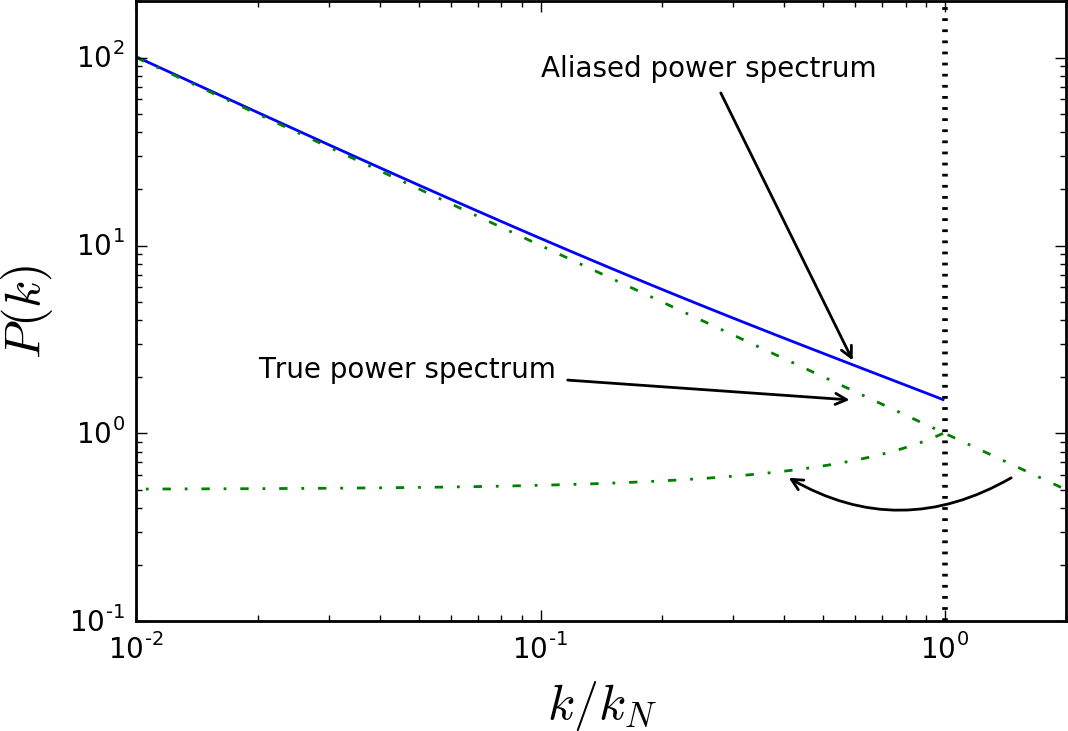
\includegraphics[width=0.9\columnwidth]{images/aliasingscheme.png}
%   \caption{Schematic representation of the effect of the aliasing in the linear 
% power spectrum. The original density contrast $\delta(\mathbf{x})$ is sampled 
% with a constant sampling interval (defined on a grid), then the Fourier 
% transform $\delta(\mathbf{k})$ is defined only between plus and minus the 
% Nyquist critical wavevector in each axis. Given that, power spectrum outside 
% that range is aliased into the range (Based on the Figure 12.1.1. of 
% \citet{Press1992}).}
%   \label{fig:aliasingeffect}
% \end{figure}

In order to measure the effect of the aliasing in the power spectrum and 
bispectrum, we are going to use the feature that for wavevector magnitudes 
close to the  inside Nyquist wavevector the aliasing effect is particularly 
relevant, while for wavevector magnitudes with $k\ll k_N$ the aliasing effect 
is negligible. Hence, if we compare two estimations, one in which the aliasing 
is negligible at a given range (e.g. if we choose a grid with a number 
of cells big enough), and we compare with one in which the aliasing effect is 
high, we can get a way to compare the aliasing for different mass assignment 
schemes. We are going to use this approach for this work.


\todo[inline]{Como se estima el espectro de potencia y bispectrum en los datos?
detalles de la implementacion.
Pruebas? Todo funciona bien? -> comparaciones con el modelo teorico!

Una buena descripcion para dummies de como calcular el bispectrum.}

%%%%%%%%%%%%%%%%%%%%%%%%%%%%%%%%%%%%%%%%%%%%%%%%%%%%%%%%%%%%%%%%%%%%%%
%% SECTION 3: RESULTS
%%%%%%%%%%%%%%%%%%%%%%%%%%%%%%%%%%%%%%%%%%%%%%%%%%%%%%%%%%%%%%%%%%%%%%
\section{Results} 
\label{sec:results}

\subsection{Power spectrum}
\label{sec:results:pk}

In the Figure \ref{fig:PvsCAMB}, in the upper panel we show the power spectrum estimation using the 
different schemes of this work for the grids of $512^3$ and $64^3$ cells against the result modeled 
with CAMB under the same cosmological parameters. As we can see, the values of the power spectrum 
are, in general, compatible the CAMB values. In the lower panel we show the percentage difference 
for the different schemes with respect the cells with $512^3$ and $64^3$ cells. For the NGP 
scheme we can get deviation of the order of 27\% at the $k_N$ level whereas for the CIC, TSC and 
D20 schemes we have deviations of 4\%, 1.5\% and 3.5\%, respectively, therefore, the best results 
are obtained these three MAS. 

(\textbf{Qu\'e m\'as digo???... No tengo una idea muy clara de c\'omo enfocarlo})

\begin{figure}
  \centering
  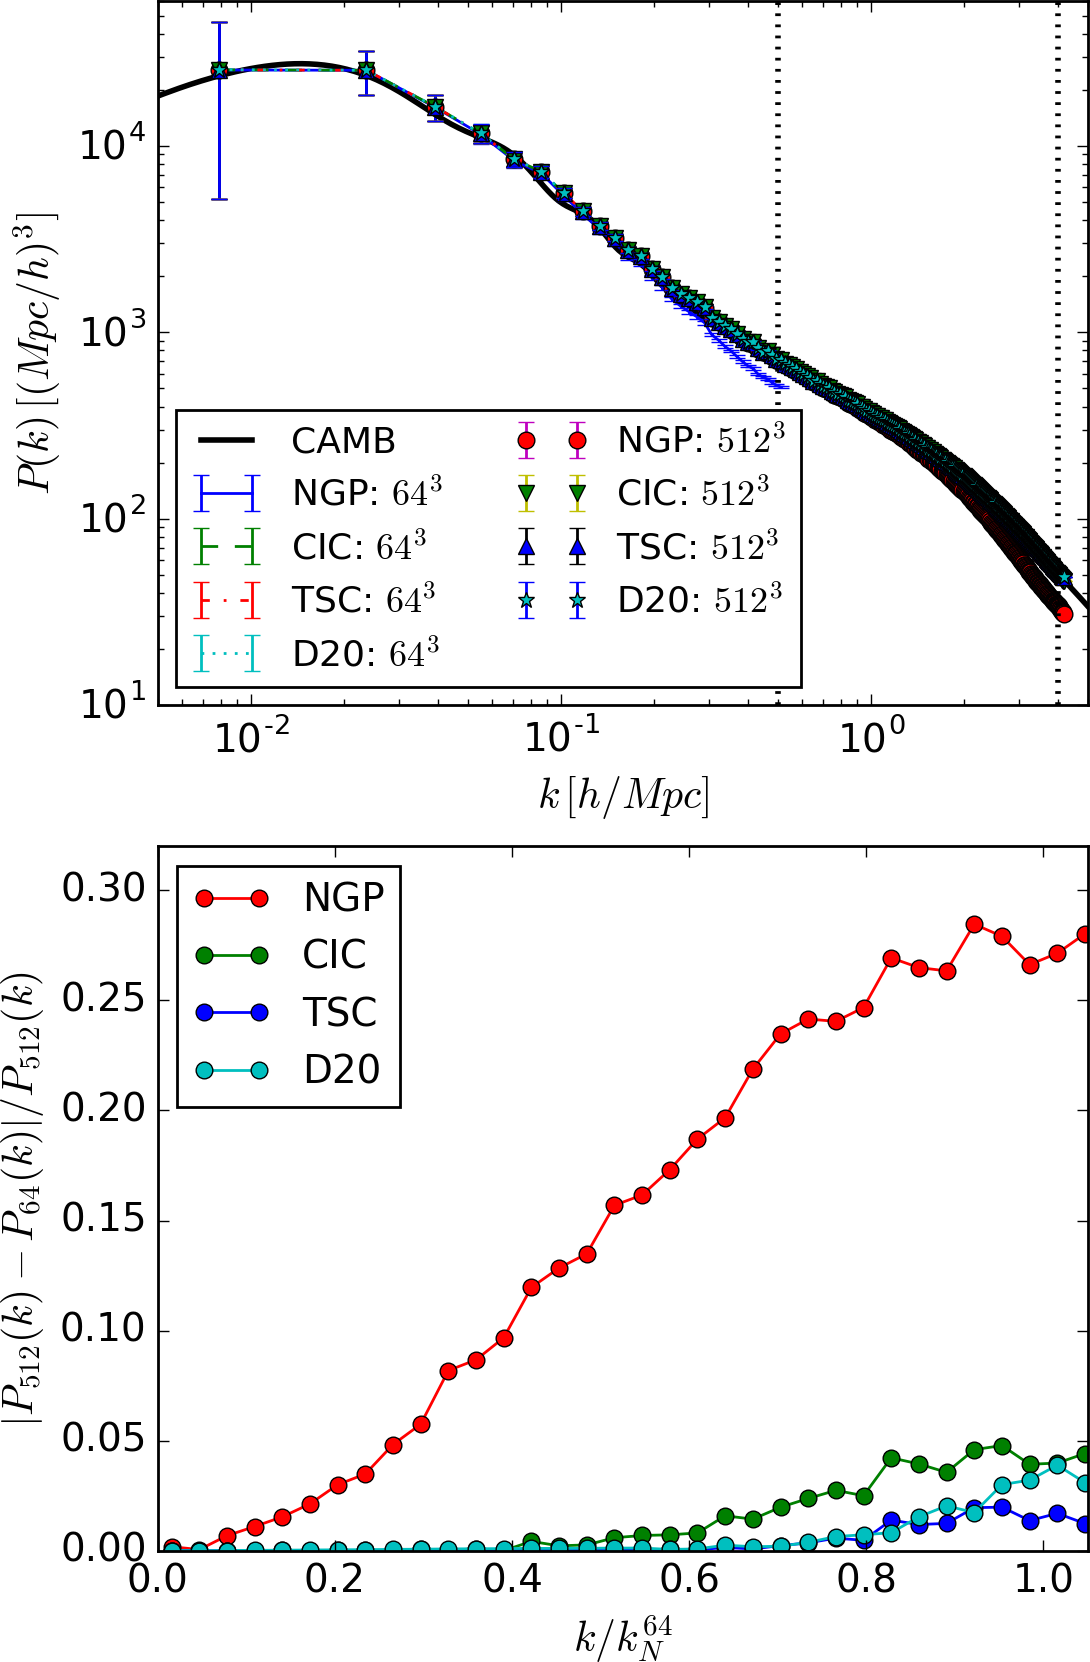
\includegraphics[width=0.95\columnwidth]{images/PowerSpectrumComparison.png}
  \caption{Graphic of the Fourier transform for the most common mass assignment schemes.}
  \label{fig:PvsCAMB}
\end{figure}



\todo[inline]{Discutir el resultado de Pk con los diferentes MAS (Colombi et.al. 2009). Efectos del 
aliasing, shot noise y demas. Como va eso en el Bk?
(figura: Pk con los diferentes MAS, mascas de kf, etc)
}

\subsection{Bispectrum}
\label{sec:results:bk}

In the Figure \ref{fig:bispectrum_plot} we show the results of the bispectrum for the grids of 
$512^3$ and $64^3$ cells. For the grid of $64^3$ we have a good match between the different values 
estimated, except for the case in which the NGP scheme was used, meaning this that is not really 
useful to use this type of MAS for the bispectrum estimation. For the other MAS we have instead that
while the wavevector get closer to the Nyquist value there is a deviation that 
not exceed the 5\% 
difference. 

%For the grid of $512^3$ cells we have instead This deviation is not noted for for the 
%grid of $512^3$ cells at least before for the cases were $k<k_N^{64}$, therefore, we can compare
%how is the proper deviation of the estimator while their are getting closer to the Nyquist 
%wavevector.

\begin{figure}
  \centering
  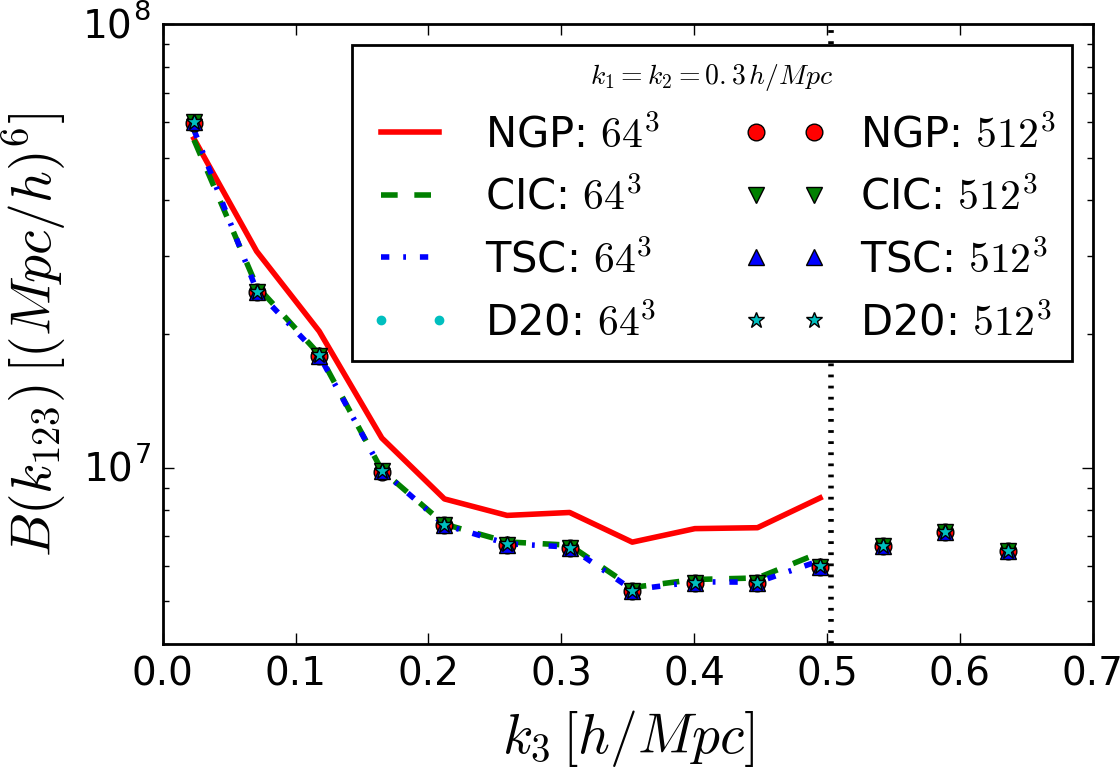
\includegraphics[width=1\columnwidth]{images/Bispectrum_plot.png}
  \caption{The aliasing effect in the power spectrum estimation for the most
  common schemes.}\label{fig:bispectrum_plot}
\end{figure}

In the upper panel of the Figure \ref{fig:BispectrumMASeffect} we show how is the percentual 
difference for the MAS with respect to their distance to the Nyquist value when the alias 
correction in the bispectrum is not made but the shotnoise term is substracted. As we can see, the 
D20 scheme has the best match with the ``non-aliased'' result but as $k_3$ side is getting closer 
to $k_N$ it can reach a percentual difference of 30\%. In the lower panel we show 
the bispectrum estimation after aliasing and shotnoise correction. As we can see after corrections 
the results improves except for the NGP scheme and getting the best results for the D20 and TSC 
schemes, were for the D20 scheme can reach a percentual difference of 1\% at the $k_N$ level.

\begin{figure}
  \centering
  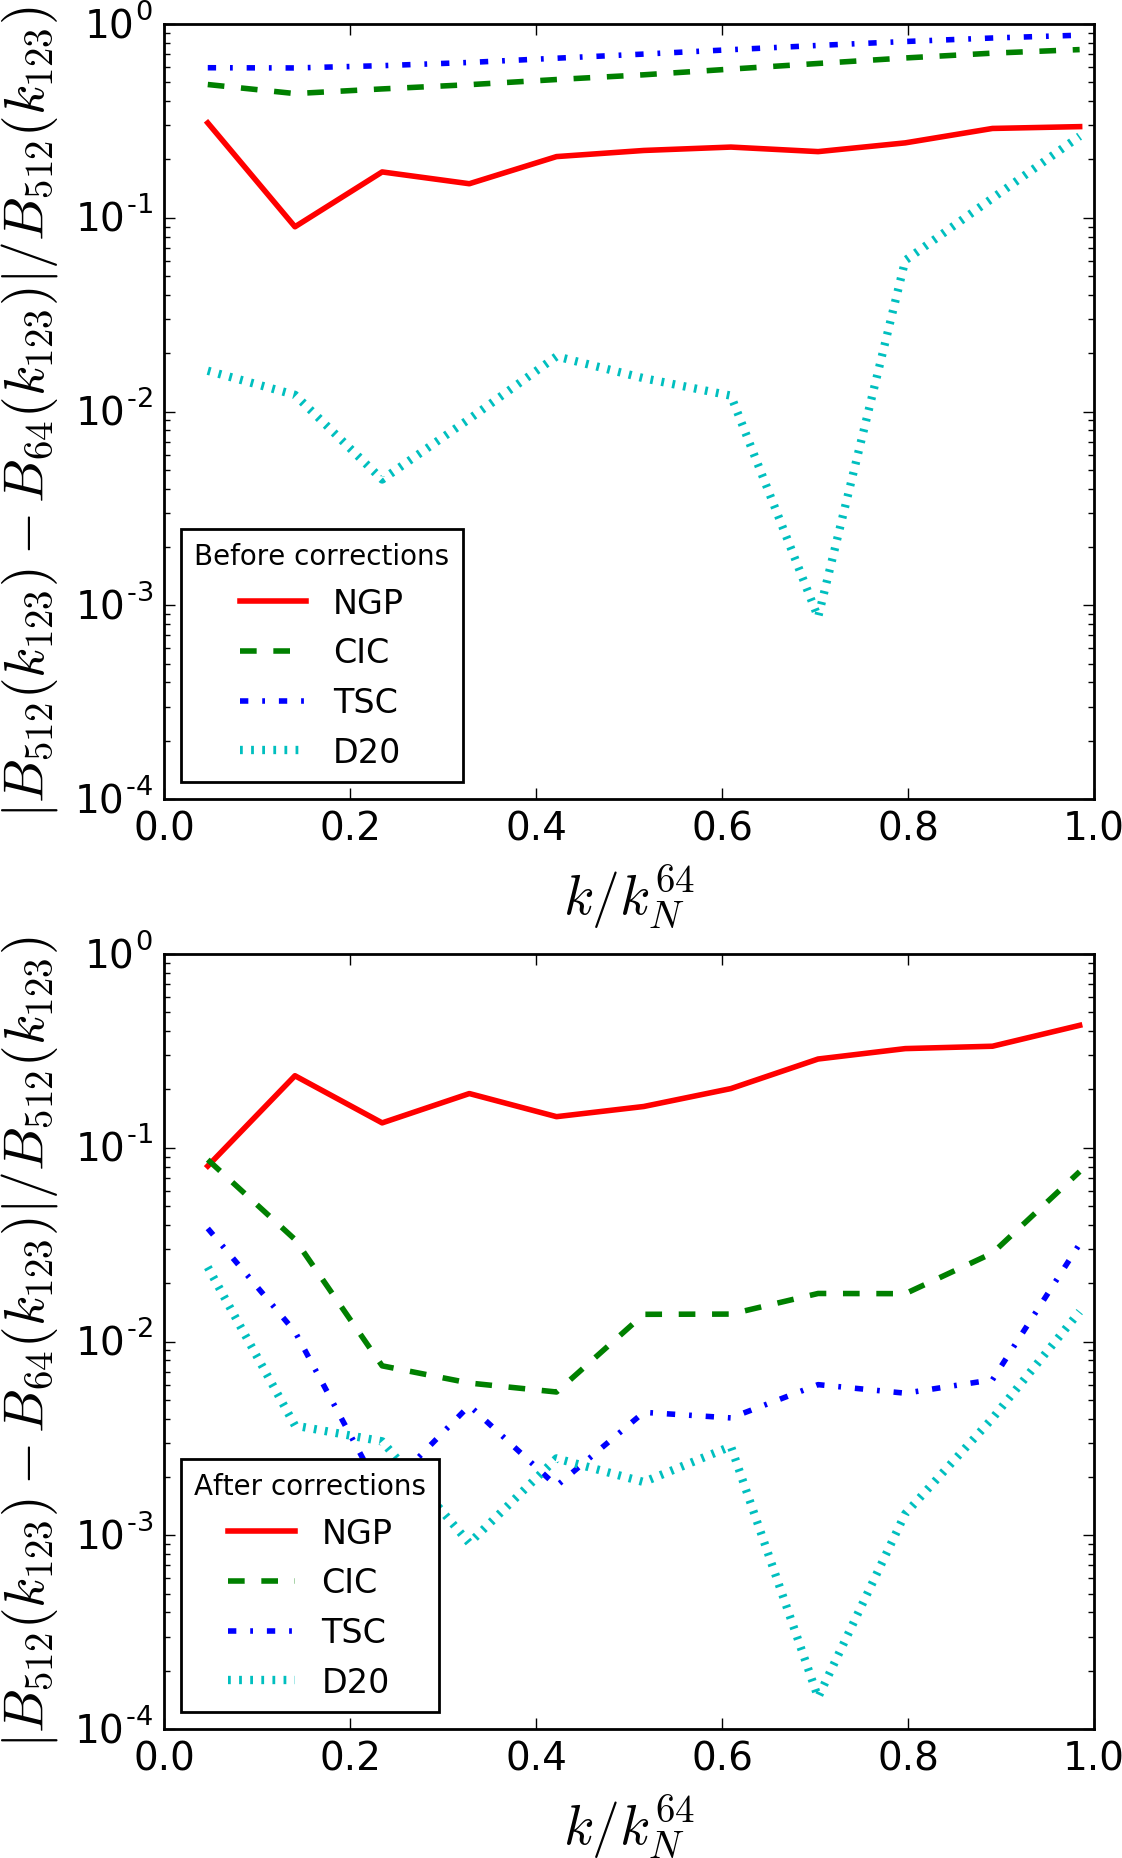
\includegraphics[width=1\columnwidth]{images/Bispectrum_CORvsNCor.png}
  \caption{The aliasing effect in the power spectrum estimation for the most
  common schemes.}\label{fig:BispectrumMASeffect}
\end{figure}

\todo[inline]{As\'i nos dio el bispectrum comparaci\'on del bispectrum con los diferentes MAS.
Analisis de diferencias.

(figura: Bk con los diferentes MAS, mascas de kf, etc)}

\subsection{Aliasing}
\label{sec:results:bk}

\todo[inline]{Estimar (cuantitativaente) los efectos del aliasing
(Figura: estimacion del aliasing, variaciones fraccionales, etc)}


\section{Summary and discussion}

In this work we use numerical simulations to study the effect of the MAS in the estimation of power 
spectrum and bispectrum. The effect of the aliasing on the power spectrum and bispectrum is 
estimated numerically in order to measure its impact on the final statistics. We show comparisons of 
different MAS in the power spectrum and bispectrum and conclude that using the standard cloud in 
cell method results in a biased bispectrum (close to 8\%) for values close the Nyquist 
wavevector. On the other hand,   the triangular shaped cloud and Daubechies 
scaling function schemes 
show the best performance with the minimum aliasing effect with relative small deviations (3\% and 
1\% respectively). We found that a MAS in the form of a Daubechies wavelet scaling function produces 
a very small aliasing effect on the bispectrum. 

Finally, we present an analytic form for the 
aliasing of the bispectrum independent of the MAS that in general provides a way to estimate the 
effect of aliasing on bispectrum estimates. This result is important, since in the current age of 
percent precision cosmology, accurate estimators of power spectrum and bispectrum are a mandatory 
tool to probe the cosmic mass density field. It is worth to mention that this is one of the first 
works studying systematically this effect on the bispectrum.


\section*{Acknowledgements}

The Acknowledgements section is not numbered. Here you can thank helpful
colleagues, acknowledge funding agencies, telescopes and facilities used etc.
Try to keep it short.

%%%%%%%%%%%%%%%%%%%%%%%%%%%%%%%%%%%%%%%%%%%%%%%%%%

%%%%%%%%%%%%%%%%%%%% REFERENCES %%%%%%%%%%%%%%%%%%

\bibliographystyle{mnras}
\bibliography{references} % if your bibtex file is called example.bib

%%%%%%%%%%%%%%%%%%%%%%%%%%%%%%%%%%%%%%%%%%%%%%%%%%

%%%%%%%%%%%%%%%%% APPENDICES %%%%%%%%%%%%%%%%%%%%%

\appendix

\section{Some extra material}

If you want to present additional material which would interrupt the flow of the main paper,
it can be placed in an Appendix which appears after the list of references.

%%%%%%%%%%%%%%%%%%%%%%%%%%%%%%%%%%%%%%%%%%%%%%%%%%


% Don't change these lines
\bsp	% typesetting comment
\label{lastpage}
\end{document}

% End of mnras_template.tex
